% Chapter 1

\chapter{Introduction} % Main chapter title

\label{Introduction2} % For referencing the chapter elsewhere, use \ref{Chapter1} 

%----------------------------------------------------------------------------------------

% Define some commands to keep the formatting separated from the content 
\newcommand{\keyword}[1]{\textbf{#1}}
\newcommand{\tabhead}[1]{\textbf{#1}}
\newcommand{\code}[1]{\texttt{#1}}
\newcommand{\file}[1]{\texttt{\bfseries#1}}
\newcommand{\option}[1]{\texttt{\itshape#1}}

%----------------------------------------------------------------------------------------
In the field of educational measurement, a test is a collection of items developed to measure students' abilities. In order to make different measurements comparable, tests should be designed and developed providing evidence of fairness, reliability and validity \parencite{AERA2014}. These ideas have evolved together with the development of new test theories but they are all based on the necessity of controlling the testing environment and procedures in such a way differences among testing conditions do not influence the scores. The test assembly is a process by which items from an item pool are selected to build test forms conforming to content and psychometric specifications. Thus, it plays a crucial role in this framework because it allows to control the entire protocol of the test production, from the item construction, since the features of the pool depend on the requirements on the final tests, to the final test building: the core of test assembly. 

Large testing programs, having better access to modern digital resources like sophisticated item banking systems, opened the possibility to improve their test assembly process by means of automated test assembly (ATA). ATA differs from manual test assembly because the item selection is performed by optimizing mathematical models through specific softwares, called solvers. Therefore, it has several advantages over manual test assembly. First of all, if the tests specifications are defined rigorously, it will reduce the need to repeat some phases of the test development. More importantly, ATA is the only way to find optimal or near-optimal combinations of items starting from large item banks, for which manual assembly is not feasible due to the large number of possible solutions. As a consequence, ATA is fundamental to make measurements comparable while reducing operational costs. 

In practice the ATA models are not always easy to solve because they involve a very large number of decision variables and constraints. Moreover, with the standard form suggested in \textcite{VDL2005} it is not possible to define any part of the model in a non-linear manner unless one resorts to approximations. Another limit of classical optimization models, until now applied for ATA, is that they consider each variable as fixed or known. This may be valid for prices, quantity of product but not for estimates, key elements in ATA models. In fact, most test assembly models are based on item response theory (IRT) which is used for estimating the item characteristics, a process called parameter calibration, and the ability of the examinees. Subsequently, IRT item parameters and the item information function (IIF) are examples of uncertain inputs in ATA models. 

\section{Main contributions}

The restrictions mentioned above motivated us to find an alternative way to specify and solve ATA models. For the first point we suggested a test assembly model based on the \emph{chance-constrained} (CC) approach \parencite[see][]{charnes1958cost} which allows to maximize the $\alpha$-quantile of the sampling distribution of the test information function (TIF). The proposed model is an extension of the classical MAXIMIN ATA model \parencite[][, p.69-70]{VDL2005} in which the minimum TIF among all the tests is maximized. The sampling distribution of the TIF is obtained by adopting the boostrap technique in the calibration process \parencite{efron1993, shao2012}. In this way we ensure that, independently on the situation in which the calibration has been made, we have an high probability to have a certain error (possibly low) in the ability estimation. For solving the ATA models, chance-constrained or not, we developed an algorithm based on a stochastic meta-heuristic called \emph{simulated annealing} (SA) proposed by \textcite{goffe1996simann}. This technique can handle large-scale models and non-linear functions. Thanks to the Lagrange relaxation and to a random variable that accepts or not an inferior solution, the useful properties of our algorithm are essentially two: it can always find the most feasible set of test forms and tries to avoid to be trapped in a local optimum seeking for the globally optimal set of test forms.

The proposed chance-constrained model, as already mentioned, is based on the empirical distribution of the TIFs of the assembled tests. This element is constructed starting from the calibration process, that is the procedure in which the IRT item parameters, such as discrimination and easiness, are estimated. More specifically, a bootstrap procedure is performed resampling the response data and generating a sample of estimates for each item parameter. At the end of this phase, the item information function (IIF) for all the items in the pool, at a predefined ability point, is computed using the bootstrapped samples. These quantities are then used in the chance-constrained model to compute the $\alpha$-quantiles of the TIFs and the model is optimized by looking for the best combination of items which produces the tests with the highest quantiles. 
The use of the bootstrap technique in the calibration is not only propaedeutic for our test assembly model but it is also a method to retrieve additional information on the variability of the item parameters without affecting their native underlying interdependence\footnote{We do not sample independently from the empirical distribution of each item parameter, instead, we resample the data following the bootstrap principle and we let the calibration algorithm produce directly the TIFs samples. This procedure should preserve the natural relationships between the item parameters.}. 

All the algorithms described in this work are coded in Julia \parencite{bezanson2017julia}, this choice has been made to achieve the best performance in numerical analysis and for the availability of many valuable and customizable packages for optimization. Two packages have been developed and are available upon request\footnote{The packages are available on github at \url{https://github.com/giadasp/IRTCalibration} and \url{https://github.com/giadasp/ATA.jl}. The first package, \texttt{IRTCalibration}, allows to calibrate an item pool following a unidimensional model with the one-parameter logistic or two-parameter logistic formulations, respectively 1PL or 2PL, estimated on dichotomous response data. \texttt{IRTCalibration} uses the techniques described in Chapter \ref{ch:Julia}. Futhermore, it provides the bootstrap tool to derive the sampling distribution functions of the item parameters. The second package, \texttt{ATA.jl}, implements the algorithms explained in Chapter \ref{ch:CC} to assemble tests optimizing the classical MAXIMIN ATA model and the proposed chance-constrained MAXIMIN ATA model.

\section{Outline of the dissertation}
The following figure gives a depicted idea of the entire framework we developed in this thesis:

\begin{figure}[H]
	\centering
	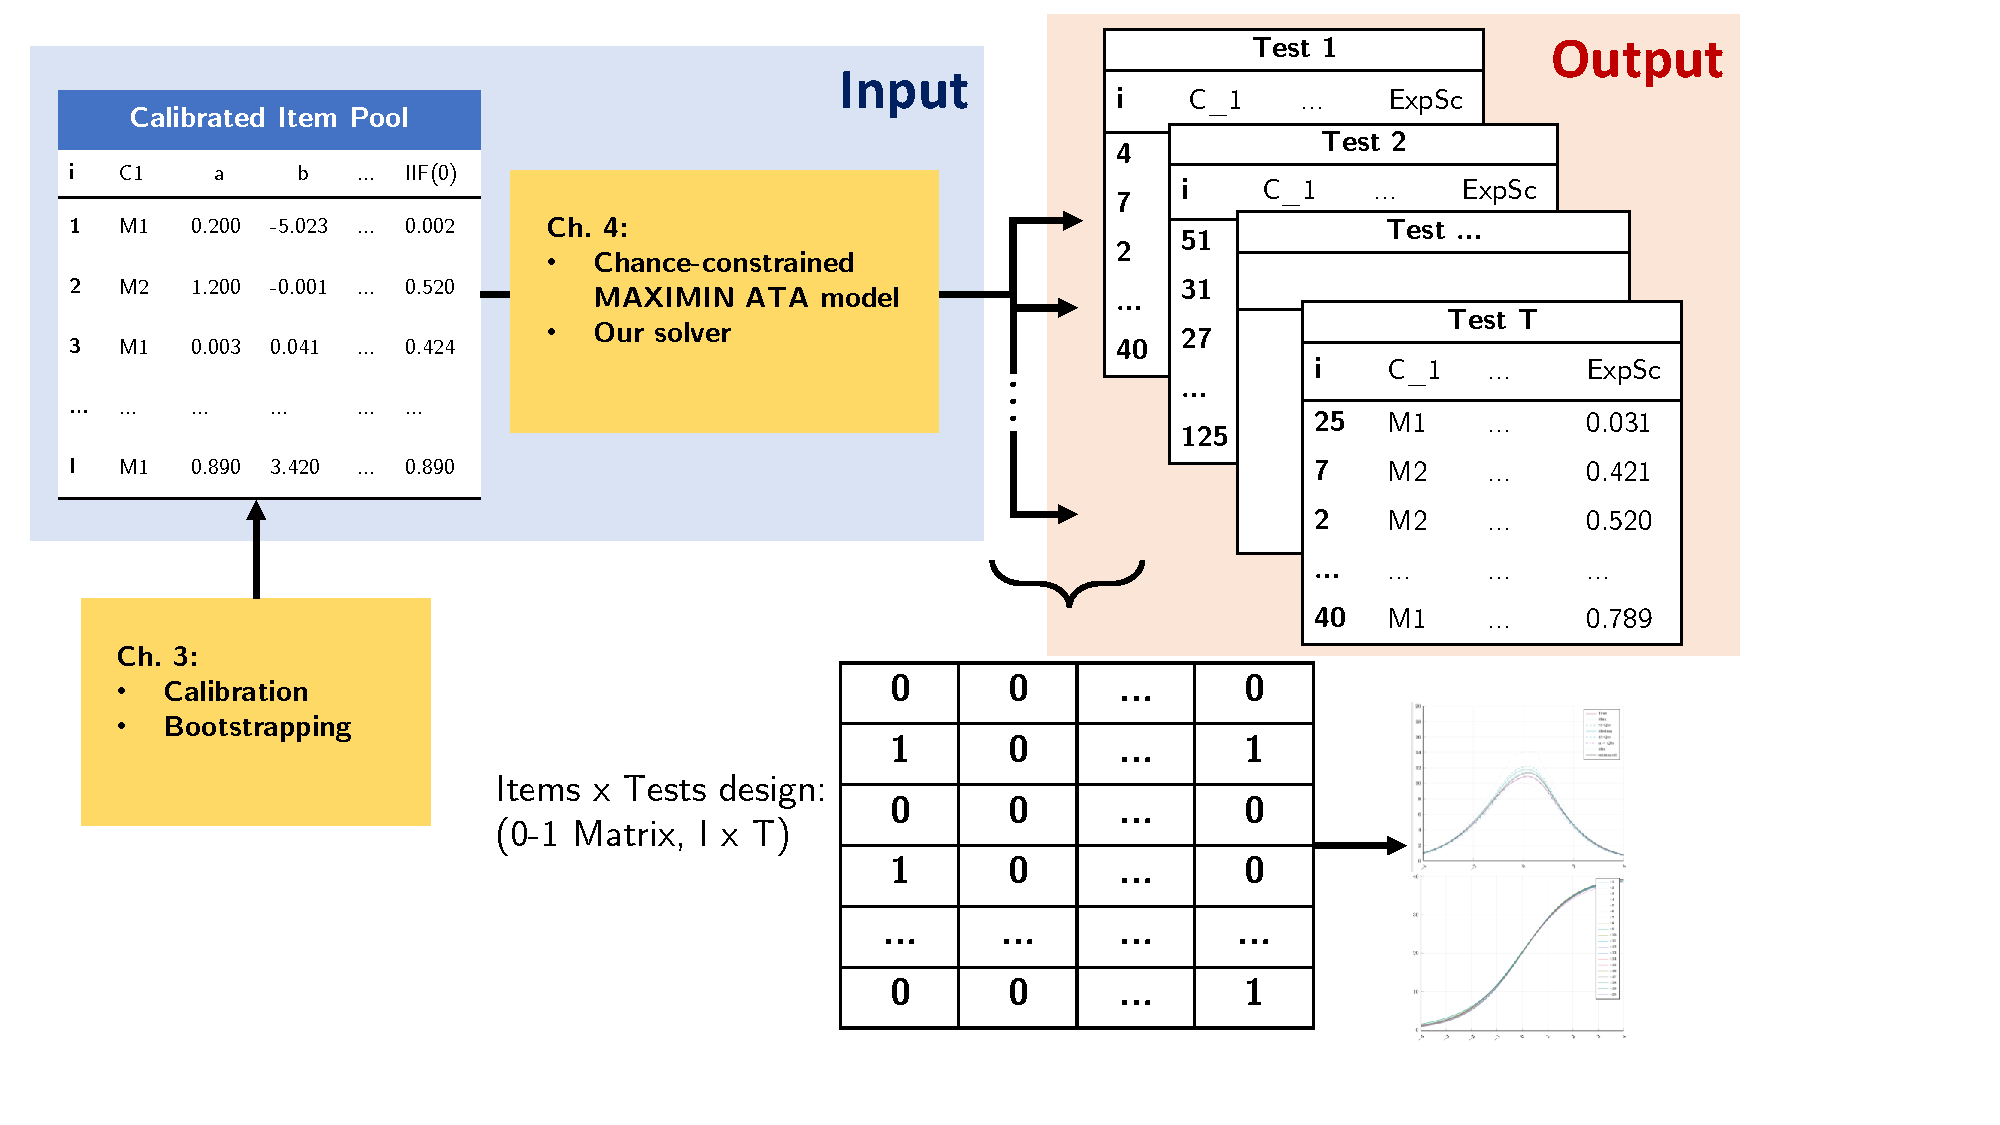
\includegraphics[width=\linewidth]{Figures/STEP3.pdf}
	\caption{Framework of the thesis, a depiction.} 
\end{figure}

Since, nowadays, several test assembly models are either based on classical test theory (CTT) or IRT, the dissertation starts, in Chapter \ref{ch:ATA}, with a brief excursus on the available test theories and continues with an introduction to the automated test assembly models. The latter topic is enriched describing the model relaxation using the Lagrange multipliers. 

It follows, in Chapter \ref{ch:Julia}, a software benchmarking, in which \texttt{Julia} is proposed as a programming language for calibrating the IRT item parameters following the 1PL and 2PL latent variable models. In this setting the empirical histogram method by \textcite{woods2007} is revised and a cubic-spline method is proposed to interpolate and extrapolate the observed distribution of the ability at predefined quadrature points. A simulation study to compare estimation accuracy and computational performance of our algorithm with respect to the \texttt{R} package \texttt{mirt} has been conducted. Moreover, both a parametric and a non-parametric bootstrap techniques are provided within the software and, taking the \emph{standard setup} defined in Section \ref{sec:semcalbs}, we illustrate the results of their application by means of a simulation study. 

In Chapter \ref{ch:CC}, the CC test assembly model is defined and a specific empirical version is proposed which allows to assemble parallel test forms in terms of percentiles of the TIFs. To solve the model the SA meta-heuristic is used. At last, the performance of the heuristic is tested in optimizing both the CC and MAXIMIN models on a simulated item pool always following the already mentioned \emph{standard setup}. At the end, we show an application of the CC MAXIMIN ATA model on real data coming from the 2018/2019 standardized assessment program of INVALSI (Italian national institute for the educational evaluation of instruction and training). This exercise is limited because the response data were available only for 39 items. However, with the aim to show that our approach is applicable to real world situations, we decided to replicate the estimates of the item parameters 8 times in order to have a richer item pool with length 312. 

Conclusions and further research ideas are provided in Chapter \ref{ch:conclusions}. 

Supplementary tables and figure, which cannot be displayed floating in the body of text are reported at the end of the essay, in Appendix \ref{ch:TablesAndFigures}.


\pagebreak